\documentclass[12pt,prb,aps]{revtex4-1}
\usepackage {amsmath}
\usepackage{amssymb}
\pdfoutput = 1 
\usepackage {graphicx}
\newcommand{\bomega}{\mbox{\boldmath$\omega$}}

\begin{document}

\title{Cylindrical Multi-Harmonic Rutherford Island Theory}

\author{R.~Fitzpatrick\,\footnote{rfitzp@utexas.edu}}
\affiliation{Institute for Fusion Studies,  Department of Physics,  University of Texas at Austin,  Austin TX 78712, USA.}

%\begin{abstract}
%\end{abstract}

\maketitle

\section{Introduction}
\section{Preliminary Analysis}
\subsection{Tokamak Equilibrium}
Consider a large aspect-ratio, low-$\beta$,  tokamak plasma equilibrium whose magnetic flux-surfaces map out (almost)
concentric circles in the poloidal plane. Such an equilibrium can be approximated as a periodic cylinder.\cite{wesson1} Let us employ a conventional set of right-handed cylindrical coordinates, $r$, $\theta$, $z$. The
equilibrium magnetic flux-surfaces correspond to surfaces of constant $r$. The system is assumed to be periodic
in the $z$ (`toroidal') direction with periodicity length
$2\pi\,R_0$, where $R_0$ is the simulated major radius of the plasma. The safety-factor profile takes the form
$q(r) = r\,B_z/[R_0\,B_\theta(r)]$, where $B_z$ is the
constant `toroidal' magnetic field-strength, and $B_\theta(r)$ is the poloidal magnetic field-strength.  Finally, the standard large aspect-ratio tokamak orderings, $r/R_0\ll 1$ and $q\sim 1$, are adopted.\cite{rf0}

\subsection{Perturbed Equilibrium}
Consider a perturbed equilibrium that is a function of
$r$, $\xi\equiv m_\theta\,\theta-n_\varphi\,\varphi$,
and time, $t$, only. Here, $m_\theta$ and $n_\varphi$ are positive integers, and $\varphi= z/R_0$ is a simulated
toroidal angle. Let ${\bf n} = (0,\,\epsilon/q_s,\,1)$,
where $\epsilon = r/R_0$ and $q_s=m_\theta/n_\varphi$. 

\subsection{Reduced-MHD Equations}
Our starting point is a set of MHD equations that neglects plasma compressibility,
but incorporates  plasma resistivity, plasma
viscosity,  and non-inductive current drive: 
\begin{align}
\nabla\cdot{\bf V} &= 0,\label{e9.1m}\\[0.5ex]
\rho\left[\frac{\partial {\bf V}}{\partial t} + ({\bf V}\cdot\nabla) {\bf V}\right]+\nabla p -{\bf j}\times {\bf B}-\mu\,\nabla^2{\bf V} &=0,\label{e9.2m}\\[0,5ex]
{\bf E} + {\bf V} \times {\bf B} &=\eta\,({\bf j}-{\bf j}_{\rm ni}).\label{e9.3m}
\end{align}
Here, ${\bf V}$, $\rho$, $p$,   ${\bf j}$, ${\bf B}$,  $\mu$, ${\bf E}$, $\eta$, and ${\bf j}_{\rm ni}$  represent the plasma flow velocity, the plasma mass density, the plasma
pressure, the total plasma current density, 
 the magnetic field-strength,  the (anomalous perpendicular) plasma viscosity, the electric field-strength,  the plasma electrical resistivity, and the non-inductive component of the plasma current density, respectively.  The  mass density  and viscosity are  assumed to be spatially uniform, for the sake of simplicity.  
Equations (\ref{e9.1m})--(\ref{e9.3m})  form a complete set when combined with the following subset of 
Maxwell's equations:
$\nabla\cdot{\bf B} =0$,
$ \nabla\times {\bf E}=-\partial{\bf B}/\partial t$, and $\nabla\times {\bf B} = \mu_0\,{\bf j}$.
 
We can automatically satisfy Eq.~(\ref{e9.1m}) and
$\nabla\cdot{\bf B}=0$ by writing
${\bf V} = \nabla\phi\times {\bf n} + V_z\,{\bf n}$ and ${\bf B} = \nabla\psi\times {\bf n} + B_z\,{\bf n}$, respectively. 
If we take the scalar product of Eq.~(\ref{e9.3m}) with ${\bf n}$, and the scalar product of the curl of Eq.~(\ref{e9.2m}) with ${\bf n}$, making use of
Maxwell's equations, then we obtain the reduced-MHD equations:\cite{strauss}
\begin{align}\label{e4}
\frac{\partial\psi}{\partial t} &= [\phi,\psi] +\frac{\eta}{\mu_0}\,(J + J_{\rm ni}) + E_z,\\[0.5ex]
\rho\,\frac{\partial U}{\partial t}&=\rho\,[\phi,U] + \mu_0^{-1}\,[J,\psi]+\mu\,\nabla^2 U,\\[0.5ex]
J & = \nabla^2\psi - \frac{2\,B_z}{R_0\,q_s},\\[0.5ex]
U &=\nabla^2 \phi,\label{e7}
\end{align}
where $[A,B]\equiv \nabla A\times \nabla B\cdot{\bf n}$.
Here, $J_{\rm ni} = \mu_0\,{\bf n}\cdot{\bf j}_{\rm ni}$, 
and $E_z$ is the constant (in $r$) inductive electric
field that maintains the equilibrium toroidal plasma current. 

\subsection{Plasma Equilibrium}
The unperturbed plasma equilibrium is specified by 
\begin{align}
\psi(r) &= \frac{B_z}{R_0\,q_s}\int_{r_s}^r r'\left[1- \frac{q_s}{q(r')}\right]dr',\\[0.5ex]
J(r) &= -\frac{B_z}{R_0}\,{\cal J}(r),\\[0.5ex]
J_{\rm ni}(r)&= \frac{B_z}{R_0}\,{\cal J}_{\rm ni}(r),\\[0.5ex]
\phi(r)&= - \frac{V_\theta'}{2}\,r^2,\\[0.5ex]
U &= - 2\,V_\theta',
\end{align}
where
\begin{align}
{\cal J}(r) &= \frac{2-s}{q},\\[0.5ex]
s(r) &= \frac{r\,q'}{q},
\end{align}
and $'\equiv d/dr$. Here, $r_s$ is the minor radius of the so-called resonant surface, defined by $q(r_s)=q_s$,
at which ${\bf k}\cdot{\bf B}=0$, where ${\bf k}$ is the wavenumber of the perturbation, and ${\bf B}$ is the equilibrium magnetic field. Note that we are assuming that the plasma is rotating as a solid body (i.e., $V_\theta'$ is independent of $r$), for the sake of simplicity. 

\subsection{Linearized Reduced-MHD Equations}
When the  perturbation is taken into account,
we can write
\begin{align}\label{e16}
\psi(r,\xi,t) &= \frac{B_z}{R_0\,q_s}\int_{r_s}^r r'\left[1- \frac{q_s}{q(r')}\right]dr' + \sum_{m=1,\infty}\psi_m(r)\,{\rm e}^{\,{\rm i}\,(m\,\xi+\gamma\,t)},
\\[0.5ex]
J(r,\xi,t) &= -\frac{B_z}{R_0}\,{\cal J}(r) +  \sum_{m=1,\infty}J_m(r)\,{\rm e}^{\,{\rm i}\,(m\,\xi+\gamma\,t)},\\[0.5ex]
J_{\rm ni}(r,\xi,t)&= \frac{B_z}{R_0}\,{\cal J}_{\rm ni}(r),\\[0.5ex]
\phi(r,\xi,t) &= - \frac{V_\theta'}{2}\,r^2 +  \sum_{m=1,\infty}\phi_m(r)\,{\rm e}^{\,{\rm i}\,(m\,\xi+\gamma\,t)},\\[0.5ex]
U(r,\xi,t) &= -2\,V_\theta' + \sum_{m=1,\infty}U_m(r)\,{\rm e}^{\,{\rm i}\,(m\,\xi+\gamma\,t)}.\label{e19}
\end{align}

Substituting Eqs.~(\ref{e16})--(\ref{e19}) into the
reduced-MHD equations, (\ref{e4})--(\ref{e7}), and only
retaining terms that are first order in small
quantities, we obtain the  linearized reduced-MHD equations:
\begin{align}\label{e20}
\gamma'\,\psi_m&= -{\rm i}\,m\,m_\theta\,\frac{B_z}{R_0}\left(\frac{1}{q_s}-\frac{1}{q}\right)\phi_m  + \frac{\eta}{\mu_0}
\,\nabla^2 \psi_m,\\[0.5ex]
\gamma'\,\rho\,\nabla^2\phi_m&= -{\rm i}\,\mu_0^{-1}\,m\,m_\theta\,\frac{B_z}{R_0}\left[\left(\frac{1}{q_s}-\frac{1}{q}\right)\nabla^2+\frac{{\cal J}'}{r}\right]\psi_m+\mu\,\nabla^2\nabla^2\phi_m,\label{e21}
\end{align}
where $\gamma' = \gamma + {\rm i}\,m\,m_\theta\,V_\theta'$,
and
\begin{equation}
\nabla^2 \equiv \frac{d^2}{dr^2} + \frac{1}{r}\,\frac{d}{dr} - \frac{m^2\,m_\theta^2}{r^2}.
\end{equation}

It is helpful to define the Alfv\'{e}n timescale, 
$\tau_{A\,m} = [R_0/(m\,n_\varphi)]\,(\mu_0\,\rho/B_z^{\,2})^{1/2}$, 
the resistive diffusion timescale,
$\tau_R = \mu_0\,r_s^{\,2}/\eta$,
the momentum confinement timescale,
$\tau_M =r_s^{\,2}\,\rho/\mu$,
 the Lundquist number,
$S_m = \tau_R/\tau_{A\,m}$,
and the magnetic Prandtl number,
$P_m =\tau_R/\tau_M$.

Let $\hat{r}=r/r_s$, $\gamma'= \hat{\gamma}/\tau_{A\,m}$, 
$\psi_m = (B_z\,r_s^2/R_0\,q_s)\,\hat{\psi}_m$, and
$\phi_m = {\rm i}\,[\gamma\,r_s^2/(m\,m_\theta)]\,\hat{\phi}_m$. The normalized versions of the
linearized reduced-MHD equations, (\ref{e20}) and (\ref{e21}), become
\begin{align}
S_m\,\hat{\gamma}\left[\hat{\psi}_m - \left(1-\frac{q_s}{q}\right)\hat{\phi}_m\right]
&= \hat{\nabla}^2\hat{\psi}_m,\label{e9.27}\\[0.5ex]
\hat{\gamma}^2\,\hat{\nabla}^2\hat{\phi}_m- \frac{\hat{\gamma}\,P_m}{S_m}\,\hat{\nabla}^2\,\hat{\nabla}^2\hat{\phi}_m&= 
\left[\left(1-\frac{q_s}{q}\right)\hat{\nabla}^2+\frac{q_s\,r_s\,{\cal J}'}{\hat{r}}\right]\hat{\psi}_m,\label{e9.28}
\end{align}
where 
\begin{equation}
\hat{\nabla}^2\equiv \frac{d^2}{d\hat{r}^2}+\frac{1}{\hat{r}}\,\frac{d}{d\hat{r}}-\frac{m^2\,m_\theta^2}{\hat{r}^2}.
\end{equation}
Our normalization scheme is designed such that, throughout the bulk of the plasma, $\hat{\psi}_m\sim \hat{\phi}_m$, and the only other quantities in the previous two equations whose magnitudes differ substantially from unity are $S_m$ and $\hat{\gamma}$.
Note that we are assuming that $S_m\gg 1$ and $P_m\sim 1$.

\subsection{Asymptotic Matching}
Suppose that the perturbation   grows on a timescale that is much less than $\tau_R$, but much greater than
$\tau_{A\,m}$. It follows that
$\hat{\gamma} \ll 1 \ll S_m\,\hat{\gamma}$,
which also implies that $\hat{\gamma}\,P_m/S_m\ll 1$. 
Thus, throughout the bulk of the plasma, we can neglect the right-hand side of Eq.~(\ref{e9.27}), and the left-hand side of Eq.~(\ref{e9.28}), which is equivalent to the neglect of plasma resistivity, viscosity,  and inertia. In this case,
Eqs.~(\ref{e9.27}) and (\ref{e9.28}) reduce to the linearized marginally-stable ideal-MHD equations:\cite{fkr}
\begin{align}
\hat{\phi}_m &= \frac{\hat{\psi}_m}{1-q_s/q},\label{e9.30}\\[0.5ex]
\hat{\nabla}^2\hat{\psi}_m + \frac{r_s\,{\cal J}'\,\hat{\psi}_m}{\hat{r}\,(1/q_s-1/q)}&=0
.\label{e9.31}
\end{align}
Equation~(\ref{e9.30}) is equivalent to the well-known flux-freezing constraint,\cite{fried} and forbids any changes in the
topology of the equilibrium magnetic field-lines. 
However, it is clear that the linearized marginally-stable ideal-MHD  equations break down in the
immediate vicinity of the resonant surface. This follows from Eq.~(\ref{e9.30}), which implies that $\skew{3}\hat{\phi}_m\rightarrow\infty$ as $r\rightarrow r_s$ if $\hat{\psi}_m(0)\neq 0$ (i.e., if the topology of the magnetic
field-lines changes in the  vicinity of the resonant surface). 
 In general, we need to employ the full set of reduced-MHD equations in the so-called  inner region, close to the resonant
surface, where Eqs.~(\ref{e9.30}) and (\ref{e9.31}) break down. The remainder of the plasma,
which is governed by the linearized marginally-stable ideal-MHD  equations, is known as the  outer region. 
 
The stability problem reduces to solving the  reduced-MHD equations, (\ref{e4})--(\ref{e7}), in the inner region, solving the linearized marginally-stable ideal-MHD
equations, (\ref{e9.30}) and (\ref{e9.31}), in the outer region, and matching the two solutions at the boundary between the
inner and outer regions.\cite{fkr} In general, the solution of the so-called cylindrical tearing mode equation, (\ref{e9.31}),\cite{rf0} that satisfies
physical boundary conditions at $r=0$ and $r=a$, where $a$ is the plasma minor radius, has a gradient discontinuity across the resonant surface.\cite{fkr} 
 It is helpful to define the tearing stability
index,\cite{fkr} 
\begin{equation}\label{e25}
{\mit\Delta}_m' =\left[\frac{r_s}{\hat{\psi}_m}\,\frac{d\hat{\psi}_m}{dr}\right]_{r_{s-}}^{r_{s+}}.
\end{equation}
This  dimensionless quantity is uniquely determined by the cylindrical tearing mode equation, and the boundary conditions,
for each harmonic number, $m$. 

Let $W_1\ll r_s$ be the thickness (in $r$) of the inner region. Our task is thus to solve the   reduced-MHD equations, (\ref{e4})--(\ref{e7}), in the inner region,  subject to the matching 
condition [see Eqs.~(\ref{e16}) and (\ref{e25})]
\begin{align}\label{e26}
\psi(x,\xi,t) &\rightarrow \frac{B_z\,s_s}{R_0\,q_s}\,\frac{x^2}{2} +\sum_{m=1,\infty}
{\mit\Psi}_m(t)\left[1+\frac{1}{2}\,{\rm Re}({\mit\Delta}_m')\,\frac{|x|}{r_s}\right]\cos(m\,\xi-\varphi_m)\nonumber\\[0.5ex]
&\phantom{=} -\sum_{m=1,\infty}{\mit\Psi}_m(t)\left[\frac{1}{2}\,{\rm Im}({\mit\Delta}_m')\,\frac{|x|}{r_s}\right]\sin(m\,\xi-\varphi_m)
\end{align}
as $|x|/W_1\rightarrow\infty$. Here, $x=r-r_s$, $s_s=s(r_s)$, and the ${\mit\Psi}_m$ and $\varphi_m$ are real. 

\section{Multi-Harmonic Neoclassical Rutherford Island Theory}
\subsection{Introduction}
In this section, we shall develop the theory of a multi-harmonic neoclassical tearing mode interacting with non-inductive RF current drive.

\subsection{Normalization Scheme}
Let $\hat{x}=x/r_s$, $t=\tau_{R\,s}\,\hat{t}$, $\tau_{R\,s} = \mu_0\,r_s^{\,2}/\eta_s$, $\eta_s=\eta(r_s)$, $\psi = [B_z\,s_s\,r_s^{\,2}/(R_0\,q_s)]\,\hat{\psi}$, ${\mit\Psi}_m = [B_z\,s_s\,r_s^{\,2}/(R_0\,q_s)]\,\hat{\mit\Psi}_m$,
$J = [B_z\,s_s/(R_0\,q_s)]\left(1-2/s_s+\hat{J}\right)$, 
$J_{\rm ni} = [B_z\,s_s/(R_0\,q_s)]\,\hat{J}_{\rm ni}$, $\phi= [r_s^2/(m_\theta\,\tau_{R\,s})]\,\hat{\phi}$, and $U= [1/(m_\theta\,\tau_{R\,s})]\,\hat{U}$. 
Furthermore, let
\begin{equation}
E_z = \frac{\eta_s}{\mu_0}\,\frac{B_z}{R_0\,q_s}\,(
2-s_s)
\end{equation}
in the inner region.
The reduced-MHD equations, (\ref{e4})--(\ref{e7}), yield
\begin{align}\label{e38}
\frac{\partial\hat{\psi}}{\partial\hat{t}} &= \{\hat{\phi},\hat{\psi}\} + (1+\delta\hat{\eta})\,\hat{J} + \left(\frac{2}{s_s}-1\right)\delta\hat{\eta} + (1+\delta\hat{\eta})\,\hat{J}_{\rm ni},\\[0.5ex]
\frac{\partial\hat{U}}{\partial\hat{t}}&= \{\hat{\phi},\hat{U}\} + S^{\,2}\,\{\hat{J},\hat{\psi}\}+P\,\frac{\partial^2\hat{U}}{\partial{\hat{x}^2}},\label{e39}\\[0.5ex]
\frac{\partial^2\hat{\psi}}{\partial \hat{x}^2}&= 1+ \hat{J},\label{e40}\\[0.5ex]
\hat{U} &= \frac{\partial^2\hat{\phi}}{\partial \hat{x}^2},\label{e41}
\end{align}
in the inner region, where
\begin{align}
\{A,B\} &\equiv \frac{\partial A}{\partial\hat{x}}\,\frac{\partial B}{\partial\xi} - \frac{\partial A}{\partial\xi}\,\frac{\partial B}{\partial\hat{x}},
\end{align}
$\delta \hat{\eta} = (\eta-\eta_s)/\eta_s$, 
$S = \tau_{R\,s}/\tau_H$,
$P = \tau_{R\,s}/\tau_M$, and
\begin{align}
\tau_H &= \frac{R_0}{s_s\,n_\varphi}\left(\frac{\mu_0\,\rho}{B_z^{\,2}}\right)^{1/2}.
\end{align}
As before, the modified Lundquist number, $S$, is assumed to be much greater than unity, whereas the
modified magnetic Prandtl number, $P$, is assumed to
be of order unity. Moreover, the
matching condition (\ref{e26}) gives
\begin{align}
\hat{\psi}(x,\xi,t) &\rightarrow \frac{\hat{x}^2}{2} +\sum_{m=1,\infty}
\hat{\mit\Psi}_m(t)\left[1+\frac{1}{2}\,{\rm Re}({\mit\Delta}_m')\,|\hat{x}|\right]\cos(m\,\xi-\varphi_m)\nonumber\\[0.5ex]
&\phantom{=} -\sum_{m=1,\infty}\hat{\mit\Psi}_m(t)\left[\frac{1}{2}\,{\rm Im}({\mit\Delta}_m')\,|\hat{x}|\right]\sin(m\,\xi-\varphi_m)\label{e46x}
\end{align}
as $|\hat{x}|/\hat{W}_1\rightarrow\infty$, where
$W_1=r_s\,\hat{W}_1$. 

\subsection{Ordering Scheme}
We are assuming that $\hat{W}_1\ll 1$. In other words, we are assuming that the radial thickness of the
inner region is much less than the plasma minor radius. In the inner region,
$\hat{t}\sim \hat{W}_1$ (as will become apparent), 
$\hat{x}\sim \hat{W}_1$, $\xi\sim 1$, $\hat{\psi}\sim \hat{W}_1^{\,2}$, $\hat{J}\sim \hat{W}_1$ (this is consistent with $|{\mit\Delta}_m'|\sim 1$), $\hat{J}_{\rm ni}\sim \hat{W}_1$ (by assumption), $\delta\hat{\eta}\sim \hat{W}_1$ (by assumption), $\hat{\phi}\sim 1$, and $\hat{U}\sim
1/\hat{W}_1^{\,2}$. 
It follows that all terms in Eqs.~(\ref{e38}) and (\ref{e41}) are of the same order of magnitude. On the
other hand, the terms involving $\hat{U}$ in Eq.~(\ref{e39}) are smaller than the other term by
a factor of, at least, $(\hat{\delta}/\hat{W}_1)^{1/6}$, where $\hat{\delta}= (P/S^2)^{1/6}$ is the normalized linear layer width.\cite{rf0} Finally, the term involving $\hat{J}$ in Eq.~(\ref{e40}) is smaller
than the other terms by a factor $\hat{W}_1$. 
Thus, assuming that $\hat{\delta}\ll \hat{W}_1\ll 1$
(i.e., the radial thickness of the inner region is much greater than the
linear layer width,  but much smaller than the
plasma minor radius), Eqs.~(\ref{e38})--(\ref{e41})
reduce to 
\begin{align}\label{e42x}
\frac{\partial\hat{\psi}}{\partial\hat{t}}&= \{\hat{\phi},\hat{\psi}\}+\hat{J} - \left(\frac{2}{s_s}-1\right)\delta\hat{\eta}
+ \hat{J}_{\rm ni},\\[0.5ex]
\{\hat{J},\hat{\psi}\} &=0,\label{e48}\\[0.5ex]
\frac{\partial^2\hat{\psi}}{\partial\hat{x}^2}&= 1.\label{e49}
\end{align}
Note that plasma inertia and viscosity have dropped
out of Eq.~(\ref{e48}). 

\subsection{Analysis}
Equation~(\ref{e49}) can be integrated, subject to the
matching condition (\ref{e46x}), to give
\begin{equation}\label{e41s}
\hat{\psi}(\hat{x},\xi,\hat{t})=\frac{\hat{x}^{2}}{2}+\sum_{m=1,\infty}\hat{\mit\Psi}_m(\hat{t})\,\cos(m\,\xi-\varphi_m)
\end{equation}
in the inner region. The previous equation is
consistent with Eq.~(\ref{e46x}) provided that
$|{\mit\Delta}_m'|\,\hat{W}_1\ll 1$ for all $m$. This
ordering is known as the constant-$\psi$ approximation,\cite{fkr} and is automatically
satisfied if $|{\mit\Delta}_m'|\sim 1$ and $\hat{W}_1\ll 1$. 

Equation~(\ref{e48}) implies that
\begin{equation}
\hat{J}= \hat{J}(\hat{\psi}).
\end{equation}
In other words, the current density in the island region is a flux-surface function (i.e., it is constant on magnetic field-lines). We shall also assume that
\begin{align}
\delta\hat{\eta}  &= \delta\hat{\eta}(\hat{\psi}),\\[0.5ex]
\hat{J}_{\rm ni} &= \hat{J}_{\rm ni}(\hat{\psi})
\end{align}
because the plasma resistivity and the non-inductive current density are both functions of the plasma temperature and pressure, which are also flux-surface functions because of the very rapid parallel transport of heat and particles that is characteristic of tokamak plasmas. (See Sect.~\ref{sthermal}.)

Equation~(\ref{e42x}) can be combined with the previous four equations to give
\begin{equation}\label{e41x}
\sum_{m=1,\infty}\frac{d\hat{\mit\Psi}_m}{d\hat{t}}\,\cos(m\,\xi-\varphi_m) = \{\hat{\phi},\hat{\psi}\}
+\hat{J}(\hat{\psi}) -\left(\frac{2}{s_s}-1\right)
\delta\hat{\eta}(\hat{\psi}) + \hat{J}_{\rm ni}(\hat{\psi}).
\end{equation}
Suppose that 
\begin{equation}\label{e42}
\frac{d\hat{\mit\Psi}_m}{d\hat{t}}=\tilde{\gamma}\,\hat{\mit\Psi}_m
\end{equation}
for all $m$. This assumption is reasonable because all  the harmonics of the tearing mode are couple together nonlinearly. Furthermore, let us write
\begin{align}
\hat{W}_1 &= 4\,\hat{\mit\Psi}_1^{1/2},\label{e43}\\[0.5ex]
X &= \frac{4\,\hat{x}}{\hat{W}_1},\label{e44}\\[0.5ex]
\hat{\psi}(\hat{x},\xi,\hat{t}) &= \hat{\mit\Psi}_1(\hat{t})\,{\mit\Omega}(\hat{x},\xi),\\[0.5ex]
\epsilon_m &= \frac{\hat{\mit\Psi}_m}{\hat{\mit\Psi}_1}.\label{e46}
\end{align}
Thus, $W_1=\hat{W}_1\,r_s$ is the full radial width of the magnetic separatrix of the island chain that would develop in the inner region if $\epsilon_m=0$ for $m>1$ (i.e., if the one-harmonic approximation were valid).  Note that the $\epsilon_m$ are independent of time. 

Equations~(\ref{e42}) and (\ref{e43}) imply that
\begin{equation}\label{e47}
\frac{d\hat{W}_1}{d\hat{t}} = \lambda,
\end{equation}
where 
$\lambda = \tilde{\gamma}\,\hat{W}_1/2$. 
Note that $\lambda\sim 1$, according to our ordering assumptions. Equations~(\ref{e41s}) and (\ref{e43})--(\ref{e46})
yield
\begin{equation}\label{e50}
{\mit\Omega}(X,\xi) = \frac{X^2}{2}+f(\xi),
\end{equation}
where
\begin{equation}
f(\xi) = \sum_{m=1,\infty} \epsilon_m\,\cos(m\,\xi-\varphi_m).
\end{equation}
Finally, Eq.~(\ref{e41x}) reduces to 
\begin{equation}\label{e51}
\frac{\lambda\,\hat{W}_1}{8}\,f(\xi)= \{\skew{3}\hat{\phi},\hat{\psi}\}+\hat{J}(\hat{\psi})-\left(\frac{2}{s_s}-1\right)\delta\hat{\eta}(\hat{\psi})+\hat{J}_{\rm ni}(\hat{\psi}).
\end{equation}

\subsection{Flux-Surface Average Operator}
According to Eq.~(\ref{e50}), 
\begin{equation}
X = s\sqrt{2\left[{\mit\Omega}-f(\xi)\right]},
\end{equation}
where $s\equiv {\rm sgn}(X)$. Now,
\begin{equation}
 \{\skew{3}\hat{\phi},\hat{\psi}\} = -\hat{x}\left.\frac{\partial\hat{\phi}}{\partial\xi}\right|_{\mit\Omega}= -\frac{\hat{W}_1}{4}\,
 s\sqrt{2\left[{\mit\Omega}-f(\xi)\right]}\,\left.\frac{\partial\hat{\phi}}{\partial\xi}\right|_{\mit\Omega}.
 \end{equation}
 The  flux-surface average operator\,\cite{ruth} is defined
 \begin{equation}\label{e54}
 \langle A({\mit\Omega},\xi)\rangle= \int_{0}^{2\pi}\frac{A({\mit\Omega},\xi)\,H({\mit\Omega},\xi)}
 {\sqrt{2\left[{\mit\Omega}-f(\xi)\right]}}\,\frac{d\xi}{2\pi},
 \end{equation}
 where
 \begin{equation}\label{e55}
 H({\mit\Omega},\xi) = \left\{
 \begin{array}{ccc} 1&~~~~~&{\mit\Omega}\geq f(\xi)\\[0.5ex]
 0 &&{\mit\Omega}< f(\xi)\end{array}\right..
 \end{equation}
 It follows that
 \begin{equation}
 \langle \{\skew{3}\hat{\phi},\hat{\psi}\}\rangle = 0,
 \end{equation}
 because $\skew{3}\hat{\phi}(\hat{x},\xi,\hat{t})$ is periodic in $\xi$, with period $2\pi$, and $\skew{3}\hat{\phi}(\hat{x},\xi,\hat{t})$
 is odd in $\hat{x}$ [so $\skew{3}\hat{\phi}(0,\
 \xi,\hat{t})=0$]. Thus, the flux-surface average of Eq.~(\ref{e51}) yields
 \begin{equation}\label{e57}
 \hat{J}({\mit\Omega}) = \frac{\lambda\,\hat{W}_1}{8}\,\frac{\langle f(\xi)\rangle}{\langle 1\rangle} +\left(\frac{2}{s_s}-1\right)\delta\hat{\eta}({\mit\Omega}) - \hat{J}_{\rm ni}({\mit\Omega}).
 \end{equation}

\subsection{Asymptotic Matching} 
According to the matching condition (\ref{e46x}),
\begin{align}
2\int_{-\infty}^\infty \int_0^{2\pi} \frac{\partial^2\hat{\psi}}{\partial \hat{x}^{\,2}}\,\cos(m\,\xi-\varphi_m)\,d\hat{x}\,\frac{d\xi}{2\pi}& = {\rm Re}({\mit\Delta}_m')\,\hat{\mit\Psi}_m,\\[0.5ex]
2\int_{-\infty}^\infty \int_0^{2\pi} \frac{\partial^2\hat{\psi}}{\partial \hat{x}^{\,2}}\,\sin(m\,\xi-\varphi_m)\,d\hat{x}\,\frac{d\xi}{2\pi}& =-{\rm Im}({\mit\Delta}_m')\,\hat{\mit\Psi}_m,\label{e59}
\end{align}
for $m=1,\infty$. 
The previous two equations can be combined with Eq.~(\ref{e40}) to give 
\begin{align}\label{e60c}
2\int_{-\infty}^\infty \int_0^{2\pi} \hat{J}({\mit\Omega})\,\cos(m\,\xi-\varphi_m)\,d\hat{x}\,\frac{d\xi}{2\pi}& = {\rm Re}({\mit\Delta}_m')\,\hat{\mit\Psi}_m,\\[0.5ex]
2\int_{-\infty}^\infty \int_0^{2\pi} \hat{J}({\mit\Omega})\,\sin(m\,\xi-\varphi_m)\,d\hat{x}\,\frac{d\xi}{2\pi}& =-{\rm Im}({\mit\Delta}_m')\,\hat{\mit\Psi}_m.\label{e61c}
\end{align}
 It is easily demonstrated that 
\begin{equation}
d\hat{x}\,d\xi = \frac{(\hat{W}_1/4)\,d{\mit\Omega}\,d\xi}{s\sqrt{2\left[{\mit\Omega}-f(\xi)\right]}}.
\end{equation}
Hence, making use of  Eq.~(\ref{e54}), Eqs.~(\ref{e60c}) and (\ref{e61c}) reduce to 
\begin{align}\label{e63}
\hat{W}_1\int_{{\mit\Omega}_{\rm min}}^\infty\hat{J}_+({\mit\Omega})\,\langle\cos(m\,\xi-\varphi_m)\rangle\,d{\mit\Omega}&= {\rm Re}({\mit\Delta}_m')\,\hat{\mit\Psi}_m,\\[0.5ex]
\hat{W}_1\int_{{\mit\Omega}_{\rm min}}^\infty\hat{J}_+({\mit\Omega})\,\langle\sin(m\,\xi-\varphi_m)\rangle\,d{\mit\Omega}&=-{\rm Im}({\mit\Delta}_m')\,\hat{\mit\Psi}_m.\label{e64}
\end{align}
Here, ${\mit\Omega}_{\rm min}$ is equal to the minimum value of $f(\xi)$. Moreover, $\hat{J}_+({\mit\Omega})$ refers to the component of $\hat{J}({\mit\Omega})$ that is even in $x$. 

\subsection{Force Balance}
The radially integrated, flux-surface averaged, poloidal electromagnetic force density acting on the
plasma in the inner region is
\begin{equation}
F_\theta = \oint\oint\int_{r_{s-}}^{r_{s+}}{\bf j}\times {\bf B}\times {\bf e}_\theta\,dr\,\frac{d\theta}{2\pi}\,\frac{d\varphi}{2\pi} =-\frac{\rho\,r_s^{\,2}}{m_\theta^2\,\tau_H^2}\oint\oint\left[\frac{\partial\hat{\psi}}{\partial\hat{x}}\right]_{-\infty}^\infty\,\frac{\partial\hat{\psi}}{\partial \theta}\,\frac{d\theta}{2\pi}\,\frac{d\varphi}{2\pi}.
\end{equation}
Making use of Eqs.~(\ref{e46x}), (\ref{e43}), and (\ref{e46}), we obtain
\begin{equation}
F_\theta = \frac{\rho\,r_s^{\,2}}{2^9\,m_\theta\,\tau_H^{\,2}}\,\hat{W}_1^{\,4}\,{\cal F}_\theta,
\end{equation}
where
\begin{equation}
{\cal F}_\theta =-\sum_{m=1,\infty}m\,\epsilon_m^2\,{\rm Im}({\mit\Delta}_m').
\end{equation}

In general, we expect the electromagnetic force acting on the inner region to be balanced by a perpendicular viscous force.\cite{rf0} Moreover, the electromagnetic force acting on the inner region cannot exceed that required to bring the plasma flow at the resonant surface to a complete halt.\cite{rf0} Thus, we expect
\begin{equation}
F_\theta \lesssim \mu\,V_\theta',
\end{equation}
which implies that
\begin{equation}
{\cal F}_\theta \lesssim V_\theta'\,\tau_c\left(\frac{\hat{\delta}}{\hat{W}_1}\right)^4,
\end{equation}
where
\begin{equation}
\tau_c = 2^9\,m_\theta\,\sqrt{S\,P}\,\tau_H.
\end{equation}
Now, we are assuming that $\hat{W}_1\gg \hat{\delta}$ (i.e., the radial width of the inner region is much greater than the linear layer width). Moreover, for a tokamak plasma with realistic (i.e., highly sub-Alfv\'{e}nic) rotation levels, we expect $V_\theta'\,\tau_c\ll 1$. Hence, we deduce that ${\cal F}_\theta\ll 1$, which
implies that ${\rm Im}({\mit\Delta}_m')\ll 1$ for all $m$. In other words, even in situations in which a net force acts on the
inner region, implying that the ${\mit\Delta}_m'$ have imaginary components, the force is sufficiently small that  $|{\rm Im}({\mit\Delta}_m')|\ll |{\rm Re}({\mit\Delta}_m')|$ for all $m$. 
Thus, it is a good approximation to treat the ${\mit\Delta}_m'$ as real quantities for the purposes of asymptotic matching. 
(In reality, the poloidal electromagnetic force is balanced by neoclassical viscosity, and it is the toroidal electromagnetic force that is balanced by perpendicular viscosity. However, this
refinement does not alter the conclusion that the imaginary components of ${\mit\Delta}_m'$ are all comparatively small.)

It follows that Eqs.~(\ref{e63}) and (\ref{e64}) can be rewritten as
\begin{align}\label{e63a}
\hat{W}_1\int_{{\mit\Omega}_{\rm min}}^\infty\hat{J}_+({\mit\Omega})\,\langle\cos(m\,\xi-\varphi_m)\rangle\,d{\mit\Omega}&= {\mit\Delta}_m'\,\hat{\mit\Psi}_m,\\[0.5ex]
\hat{W}_1\int_{{\mit\Omega}_{\rm min}}^\infty\hat{J}_+({\mit\Omega})\,\langle\sin(m\,\xi-\varphi_m)\rangle\,d{\mit\Omega}&=0,\label{e64a}
\end{align}
for all $m$. 

The only obvious way of satisfying the constraints (\ref{e64a}) is to set all of the phase angles, $\varphi_m$, equal to
one another. In fact, without loss of generality, we can set all of the phase angles equal to zero. In this case,
\begin{equation}\label{e65}
f(\xi) = \sum_{m=1,\infty} \epsilon_m\,\cos(m\,\xi),
\end{equation}
and Eqs.~(\ref{e63a}) and (\ref{e64a}) become 
\begin{align}\label{e65a}
\hat{W}_1\int_{{\mit\Omega}_{\rm min}}^\infty\hat{J}_+({\mit\Omega})\,\langle\cos(m\,\xi)\rangle\,d{\mit\Omega}&= {\mit\Delta}_m'\,\hat{\mit\Psi}_m,\\[0.5ex]
\hat{W}_1\int_{{\mit\Omega}_{\rm min}}^\infty\hat{J}_+({\mit\Omega})\,\langle\sin(m\,\xi)\rangle\,d{\mit\Omega}&=0.\label{e66}
\end{align}
Equation~(\ref{e66}) is now automatically satisfied because $\hat{J}_+({\mit\Omega})$ is an even function of $\xi$ [since ${\mit\Omega}= X^2/2+f(\xi)$ is an even function of $\xi$]. 

\subsection{Perturbed Electrical Resistivity}
Let us assume, for the sake of simplicity, that the electron
number density in the inner region takes the uniform value
$n_{e\,s}$. The electrical resistivity thus satisfies $\eta\propto
T_e^{\,-3/2}$, where $T_e$ is the electron temperature.\cite{plasma} Let $u=(T_e-T_{e\,s})/T_{e\,s}$, where $T_{e\,s} = T_e(r_s)$, and
$T_e(r)$ is the unperturbed electron temperature profile. Our ordering assumptions imply that $u\sim \hat{W}_1\ll 1$. It follows
that
\begin{equation}
\delta{\hat\eta} = (1+u)^{-3/2} - 1\simeq -\frac{3}{2}\,u.
\end{equation}

\subsection{Non-Inductive Current Density}
The non-inductive current density in the inner region is
written
\begin{equation}
j_{{\rm ni}\,z} = j_{{\rm bs}\,z} + j_{{\rm rf}\,z},
\end{equation}
where 
\begin{equation}
j_{{\rm bs}\,z} = -1.46\,\frac{q_s\,n_{e\,s}}{\sqrt{\epsilon}_s\,B_z}\,\frac{\partial T_e}{\partial r},
\end{equation}
is the bootstrap current,\cite{boot,carrera,fitz} $\epsilon_s=r_s/R_0$, and $j_{{\rm rf}\,z}$ is the non-inductive current density driven by radio-frequency electromagnetic waves absorbed by the plasma in the inner region. 
It follows that
\begin{equation}
\hat{J}_{\rm bs} \equiv \frac{\mu_0\,R_0\,q_s}{s_s\,B_z}\,j_{{\rm bs}\,z} = - 1.46\,\sqrt{\epsilon}_s\,\frac{\beta_{p\,e}}{s_s}\,\frac{\partial u}{\partial \hat{x}},
\end{equation}
where 
\begin{equation}
\beta_{p\,e} = \left(\frac{q_s}{\epsilon_s}\right)^2\,\frac{\mu_0\,n_{e\,s}\,T_{e\,s}}{B_z^{\,2}}.
\end{equation}
Note that $\hat{J}_{\rm bs}\sim \hat{W}_1$, according to our ordering scheme.

\subsection{Thermal Transport}\label{sthermal}
Steady-state perturbed thermal transport in the inner region is
governed by\,\cite{plasma}
\begin{equation}
0 = \nabla_\parallel(\chi_\parallel\,\nabla_\parallel u)+ 
\nabla_\perp(\chi_\perp\,\nabla_\perp u) + \frac{P_{\rm rf}}{n_{e\,s}\,T_{e\,s}},
\end{equation}
where $\nabla_\parallel \equiv B_z^{\,-1}\,{\bf B}\cdot\nabla$,
$\nabla_\perp = \nabla - \nabla_\parallel$, $\chi_\parallel$ is the
parallel energy diffusivity, $\chi_\perp$ is the perpendicular
energy diffusivity, and $P_{\rm rf}$ is the heating power density due to radio-frequency electromagnetic waves absorbed by the plasma in the inner region. Both $\chi_\parallel$ and $\chi_\perp$ are assumed to be uniform in the inner region, for the sake of simplicity. 
It follows that
\begin{equation}\label{e85}
0 = \left(\frac{\hat{W}_1}{\hat{W}_c}\right)^4\{\{u,{\mit\Omega}\},{\mit\Omega}\} + \frac{\partial^2 u}{\partial\hat{x}^2}+\hat{P}_{\rm rf},
\end{equation}
where
\begin{align}
\hat{W}_c &= 4\left(\frac{\chi_\perp}{\chi_\parallel}\right)^{1/4}\left(\frac{R_0}{n_\varphi\,s_s\,r_s}\right)^{1/2},\\[0.5ex]
\hat{P}_{\rm rf} &= \frac{P_{\rm rf}\,\tau_E}{n_{e\,s}\,T_{e\,s}},
\end{align}
and $\tau_E=r_s^2/\chi_\perp$ is the energy confinement time. 
Let us assume that $\hat{W}_1\gg \hat{W}_c$. In other words, the
radial extent of the inner region is sufficiently large that parallel transport is able to force the electron temperature to be a flux-surface function.\cite{fitz}
We can write
\begin{equation}
u= u_0({\mit\Omega})+\left(\frac{\hat{W}_c}{\hat{W}_1}\right)^4\,u_1({\mit\Omega},\xi).
\end{equation}
To lowest order, Eq.~(\ref{e85}) gives
\begin{equation}
0 = \{\{u_1,{\mit\Omega}\},u\} + \frac{\partial^2 u_0}{\partial\hat{x}^2}+ \hat{P}_{\rm rf}.
\end{equation}
Flux-surface averaging, we obtain
\begin{equation}
0=\left\langle \frac{\partial^2 u_0}{\partial\hat{x}^2}
\right\rangle + \langle \hat{P}_{\rm rf}\rangle,
\end{equation}
which reduces to
\begin{equation}
0=\langle X^2\rangle \,\frac{d^2u_0}{d{\mit\Omega}^2} +\langle 1\rangle\,\frac{du_0}{d{\mit\Omega}} + \frac{\hat{W}_1^2}{16}\,\langle \hat{P}_{\rm rf}\rangle.
\end{equation}

Suppose, for the sake of simplicity, that $\langle \hat{P}_{\rm rf}\rangle$ is even in $x$. 


\section*{Acknowledgements}
This research was directly funded by the U.S.\ Department of Energy, Office of Science, Office of Fusion Energy Sciences,  under  contracts DE-FG02-04ER54742 and DE-SC0021156. 

\section*{Data Availability Statement}
The data that support the findings of this study are available from the corresponding author upon reasonable request.

\section*{References}
\begin{thebibliography}{99}\baselineskip 5ex

\bibitem{wesson1} J.A.~Wesson, Nucl.\ Fusion {\bf 18}, 87 (1978).
\bibitem{rf0} R.~Fitzpatrick, Nucl.\ Fusion {\bf 33}, 1049 (1993). 
\bibitem{fkr} H.P.~Furth, J.~Killeen, and M.N.~Rosenbluth, Phys.\ Fluids {\bf 6}, 459 (1963).
\bibitem{plasma} R.~Fitzpatrick, {\em Plasma Physics: An Introduction}. CRC Press, 2014. 
%\bibitem{wesson} J.A.~Wesson, {\em Tokamaks}, 4th Edition. Oxford University Press (2011).
\bibitem{ruth} P.H.~Rutherford,  Phys.\ Fluids {\bf 16}, 1903 (1973).
%\bibitem{chang} Z.~Chang, and J.D.~Callen, Nucl.\ Fusion {\bf 30}, 219 (1990).
\bibitem{fitz} R.~Fitzpatrick, Phys.\ Plasmas {\bf 2}, 825 (1995).
\bibitem{boot} R.J.~Bickerton, J.W.~Connor, and J.B.~Taylor, Nat.\ Phys.\ Sci.\ {\bf 229} (1971).
\bibitem{carrera} R.~Carrera, R.D.~Hazeltine, and M.~Kotschenreuther, Phys.\ Fluids {\bf 29},
%899 (1986). 
%\bibitem{buttery} R.J.~Buttery, S.~G\"{u}nter, G.~Giruzzi, T.C.~Hender, D.~Howell,
%G.~Huysmans, R.J.~La\,Haye, M.~Maraschek, H.~Reimerdes, O.~Sauter,
%C.D.~Warrick, H.R.~Wilson, and H.~Zohm, Plasma Phys.\ Control.\ Fusion
%{\bf 42}, B61 (2000). 
%\bibitem{lahaye} R.J.~La\,Haye, Phys.\ Plasmas {\bf 13}, 055501 (2006). 
%\bibitem{westerhof} E.~Westerhof, Nucl.\ Fusion {\bf 30}, 1143 (1990). 
%\bibitem{bar} L.~Bard\'{o}czi, and T.E.~Evans, Phys.\ Rev.\ Lett.\ {\bf 126}, 085003 (2021).
\bibitem{strauss} H.R.~Strauss, Phys.\  Fluids {\bf 19}, 134 (1976). 
\bibitem{fried} J.P.~Freidberg, Rev.\ Mod.\ Phys.\ {\bf 54}, 801 (1982). 

\end{thebibliography}

%\newpage
%\begin{figure}
%\centerline{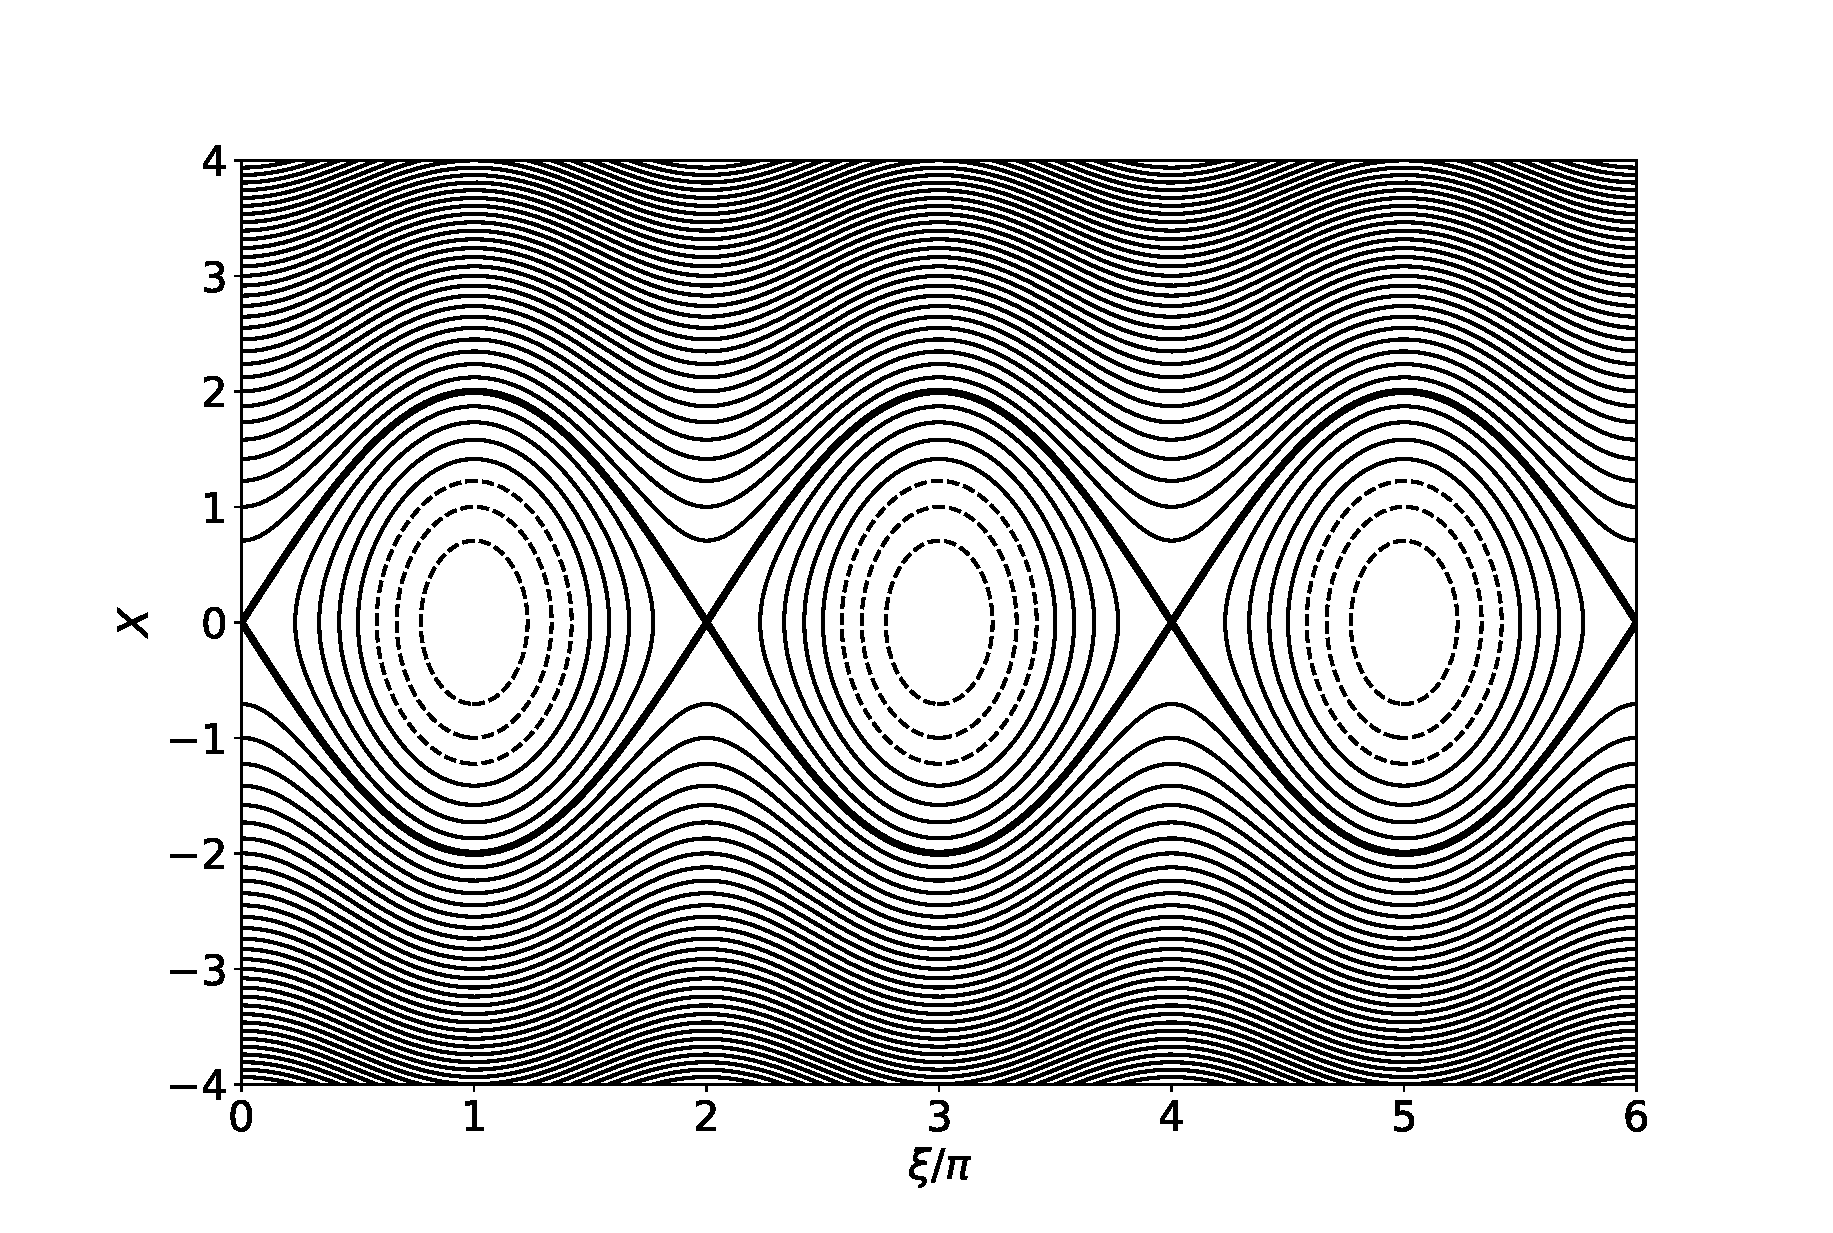
\includegraphics[height=4.5in]{Figure1.eps}}
%\caption{.}\label{fig1}
%\end{figure}


\end{document}